\chapter{Clustering Uncertainty}
Unsupervised learning algorithms may lead to unstable results due to the absence of labels. In clustering models, this instability can occur at the cluster level or even at the data point level. Indeed, from one clustering run to another, a data point might be assigned to a different cluster, especially if the training dataset is noisy or if there is no value of $K$ leading to large inter-cluster distances (separability issues).  The objective of uncertainty quantification is to be able to detect and measure instability. 

%1. Goal: detect unstable clusters and/or individual data points
%2. Issue: ensembles of clustering models cannot easily be combined/averaged
%3. Tried different approaches to compute the variability of clustering assignments

%\subsection{Data uncertainty}

To evaluate data uncertainty, a soft-clustering algorithm can produce probability scores $ p_{i,k} $ of being assigned to cluster $k$ for data point $x_i$. Under this formulation, soft-clustering is equivalent to classification with respect to uncertainty quantification. The entropy of the prediction distribution is a valid measure of data uncertainty, i.e. the instability at individual data points level for a particular clustering assignment.

% \subsubsection{Model uncertainty}

%However, the absence of  ensembles of clustering models cannot easily be 
To evaluate model uncertainty, let's consider an ensemble $ \mathcal{E} = \left\{f^m\right\}_{m = 1}^{M}$ of trained clustering models, for instance, using different initialisation seeds. Note  that $f^m(x_i)$ defines $M$ realisations for the membership probabilities $p_{i,k}^m$. A naive candidate for estimating model uncertainty for data point $x_i$ is the standard deviation of the ensemble prediction distribution.
$
U_{i,k} = \sqrt{\frac{1}{M-1} \sum_m \left (p_{i,k}^m -  \bar{p}_{i,k} \right)^2 }
$
where
\begin{equation} \label{eq:average-membership-proba}
    \bar{p}_{i,k} = \frac{1}{M} \sum_m p_{i,k}^m
\end{equation}

However, due to the intrinsic nature of clustering or, more general, unsupervised tasks, there is no guarantee that label $y^m_i$ corresponds to label $y^l_i$ when $l \not = m$. This phenomenon is referred to as label mismatch and is illustrated in figure \ref{fig:clustering-label-mismatch}. Suppose the clustering assignment is taken as reference in figure \ref{fig:clustering-label-mismatch-1}. In that case, we observe that the following label-matching function needs to be applied to be able to use equation \ref{eq:average-membership-proba}:

\begin{equation}
    k^m = g(k) = \begin{cases}
  1  \;\;, \text{if } k = 0\\
  0  \;\;, \text{if } k = 1\\
  2  \;\;, \text{if } k = 2\\
\end{cases}
\end{equation}

\begin{figure}
     \centering
     \begin{subfigure}[b]{0.49\textwidth}
         \centering
         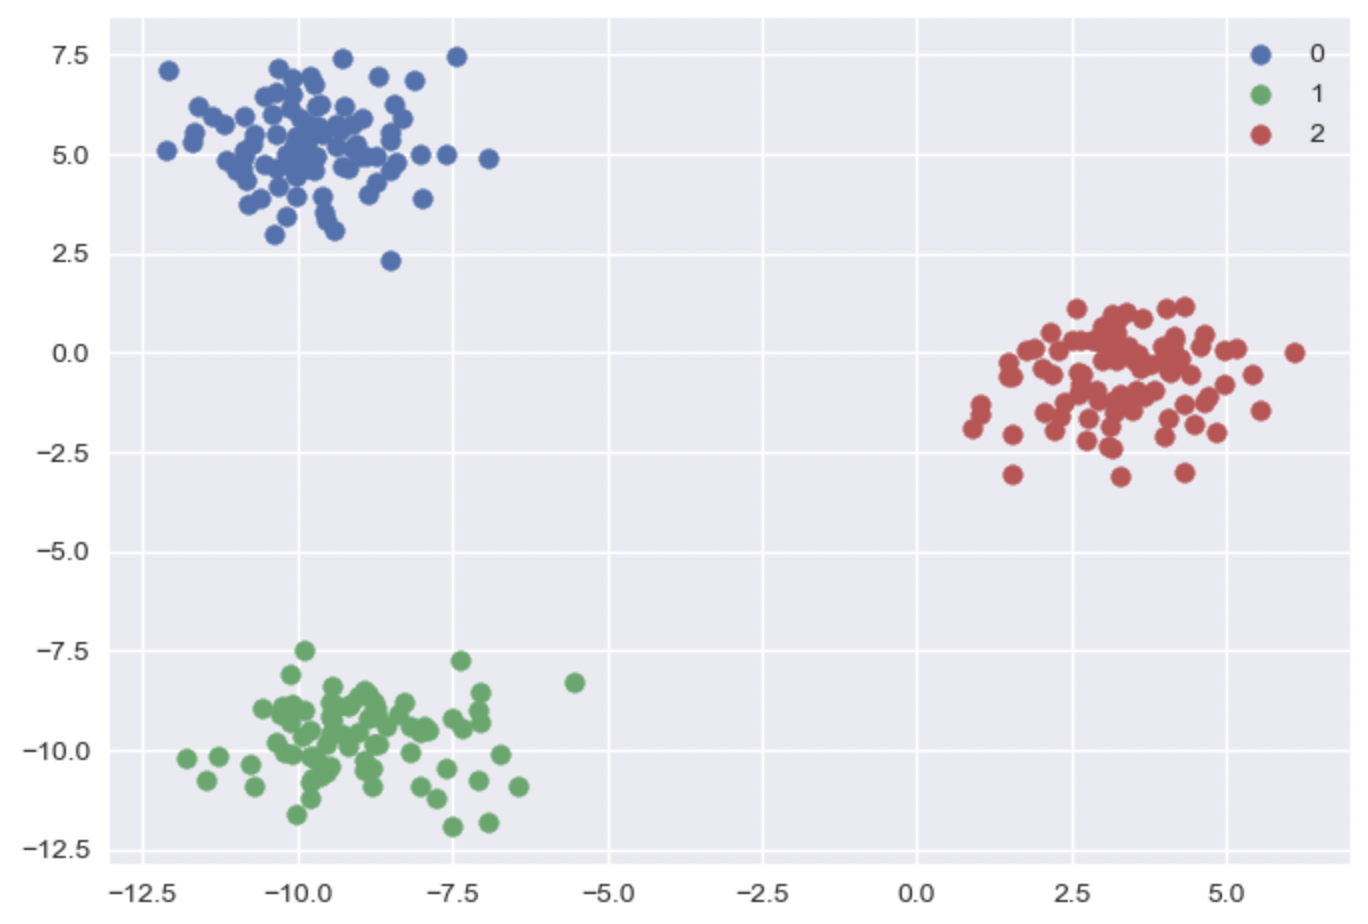
\includegraphics[width=\textwidth]{figures/design/cluster-label-switch-1.png}
         \caption{Clustering assignment (seed=0)}
         \label{fig:clustering-label-mismatch-1}
     \end{subfigure}
     \hfill
     \begin{subfigure}[b]{0.49\textwidth}
         \centering
         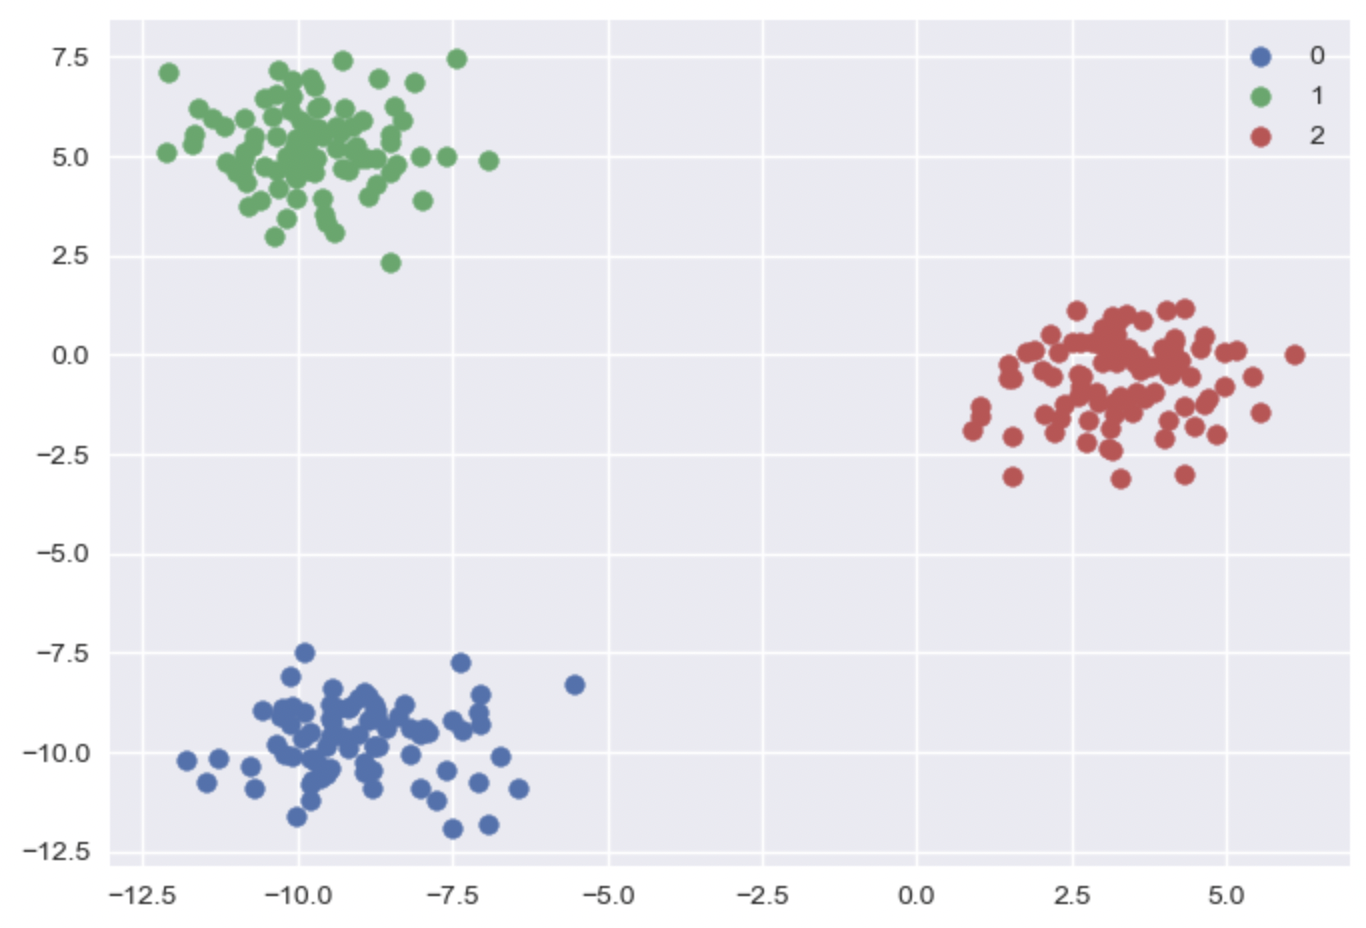
\includegraphics[width=\textwidth]{figures/design/cluster-label-switch-2.png}
         \caption{Clustering assignment (seed=1)}
         \label{fig:clustering-label-mismatch-2}
     \end{subfigure}
     \caption{Label mismatch in two clustering assignments (k=3)}
     \label{fig:clustering-label-mismatch}
\end{figure}


More generally, this implies that we do not have a single set of labels $k=0,\ldots, K-1$. Instead, we have $M$ different label combinations, represented by $k^m=0, \ldots, K-1 \; \forall \; m = 0, \ldots, M-1$. Let's consider a matching algorithm between 2 clustering models $m,l$:
$g^{m,l}(k^l) = k^m$ and its soft relaxation defined by the probability distribution 
$
 \left\{ P \left[k^l = k^m \mid m,l \right] \right\}_{k^m=0}^{K-1} =   \left\{ G^{m,l}_{k^m, k^l} \right\}_{k^m=0}^{K-1}
$
so that $g(k^l)^{m,l} = argmax_{j} \; G^{m,l}_{j, k^l}$ with the constraints $ \sum_{k^m} G^{m,l}_{k^m, k^l} = 1$, $G^{m,m}_{k^m, k^l} = 1$ when $k = k^m$ and $ G^{m,m}_{k^m, k^l} = 0 $ when $k \not= k^m$. This leads once again to a reformulation of equation \ref{eq:average-membership-proba}:

\begin{equation} 
    \tilde{\bar{p}}_{i,k} 
    = \frac{1}{M} \sum_m p_{i,k^m}^m = 
    \frac{1}{M} \sum_m  \sum_{k}  G^{m,l}_{k^m, k^l} p_{i,k}^m
\end{equation}


Let's pick a referential clustering assignment $l=0$ and redefine the average membership probabilities for the ensemble as follows:

\begin{equation} 
    \tilde{\bar{p}}_{i,k}^0 = \frac{1}{M} \sum_{m,k^m}  G^{m,0}_{k^m, k^l}  \cdot p_{i,k}^m = \frac{1}{M} \left(p_{i,k}^0 + \sum_{m>0,k^m}  G^{m,0}_{k^m, k^l}  \cdot p_{i,k}^m \right)
\end{equation}

We can further abstract the choice of referential $l=0$ by averaging over the possible values of $l$

\begin{equation} 
    \tilde{\bar{p}}_{i,k} = \frac{1}{M} \sum_l \tilde{\bar{p}}_{i,k}^l = \frac{\bar{p}_{i,k}}{M} + \frac{1}{M^2} \sum_{m\not=l,k^m}  G^{m,l}_{k^m, k^l}  \cdot p_{i,k}^m
\end{equation}
or in equivalent matrix notation $ \tilde{\bar{p}}_{i,k} = \frac{1}{M^2} \left\lVert \boldsymbol{G}_k \cdot \boldsymbol{p}_i \right\lVert_1$ where $\boldsymbol{G}_k$ has shape $M \times M \times K$

The motivation for introducing the soft matching relaxation is illustrated in figure \ref{fig:clustering-soft-matching}. In this example, the true underlying number of clusters is probably $k=3$. However, with a wrong choice for this hyper-parameter, i.e. $k=4$, we observe a cluster split phenomenon which translates to higher uncertainty for the model.

\begin{figure}
     \centering
     \begin{subfigure}[b]{0.49\textwidth}
         \centering
         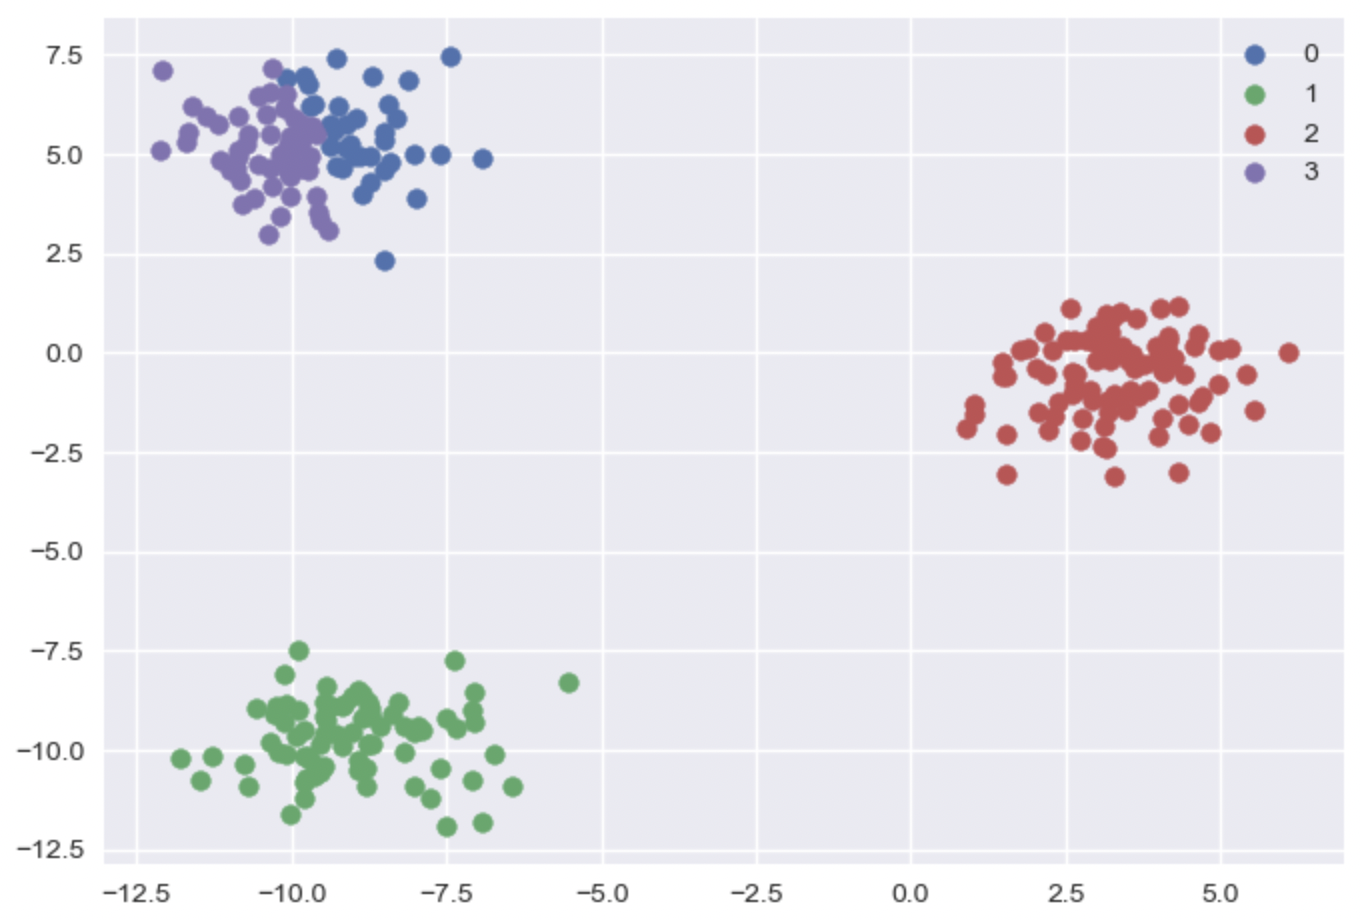
\includegraphics[width=\textwidth]{figures/design/cluster-soft-matching-1.png}
         \caption{Clustering assignment (seed=0)}
         \label{fig:clustering-soft-matching-1}
     \end{subfigure}
     \hfill
     \begin{subfigure}[b]{0.49\textwidth}
         \centering
         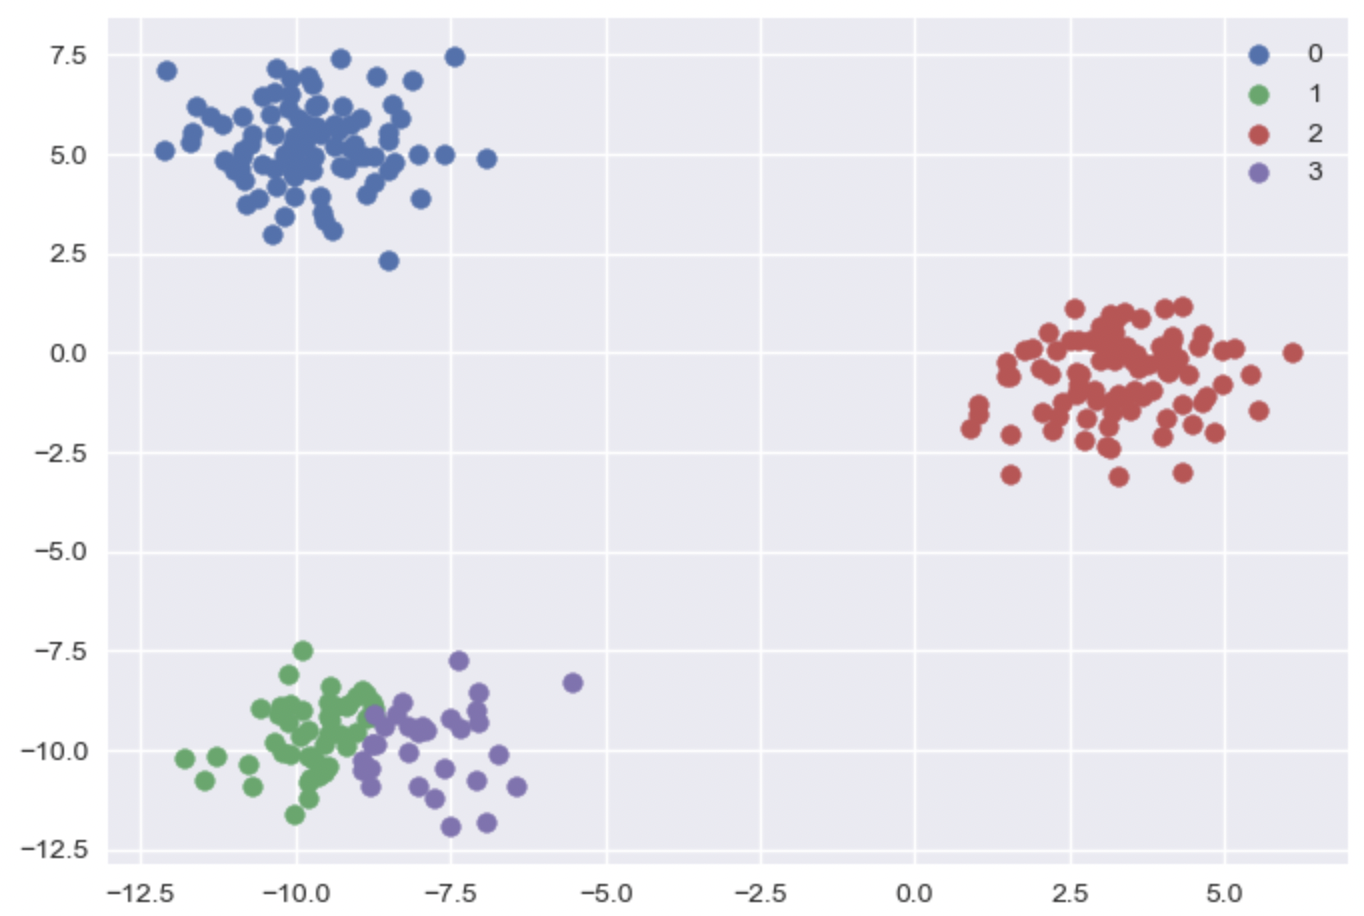
\includegraphics[width=\textwidth]{figures/design/cluster-soft-matching-2.png}
         \caption{Clustering assignment (seed=1)}
         \label{fig:clustering-soft-matching-2}
     \end{subfigure}
     \caption{Overfitting clustering assignment,  $k=4$}
     \label{fig:clustering-soft-matching}
\end{figure}

In figure \ref{fig:clustering-soft-matching-2}, cluster $0$ correspond to the union of clusters $0$ and $3$ in figure \ref{fig:clustering-soft-matching-1}. In other words, we need the soft matching relaxation to be able to place half the mass of the union cluster into the split clusters, which corresponds to the following matrix:

\begin{equation}
   \boldsymbol{G}^{1,0} = 
   \begin{bmatrix}
    1/2 & 0 & 0 & 1/2 \\
    0 & 1 & 0 & 0\\
    0 & 0 & 1 & 0 \\
    0 & 1 & 0 & 0
    \end{bmatrix}
\end{equation}

Finally, we need to discuss how to choose the matching algorithm. I propose to use the inverse $l_2$ distance between centroids $\boldsymbol{c_k^m}$, normalised to achieve a valid probability distribution

\begin{equation}
    G^{m,l}_{k^m, k^l} = \frac{\frac{1}{\lVert \boldsymbol{c_k^m - c_{k^m}^l} \lVert_2}}{\sum_{k^m} \frac{1}{\lVert \boldsymbol{c_k^m - c_{k^m}^l} \lVert_2}}
\end{equation}

\subsubsection{Clustering instability for hard-clustering algorithms}

We propose another instability metric based on the idea that a stable data point should often be clustered with the same data points across different ensemble clustering assignments. Let $S_{i,j}^m = I\{a_j^m = a_i^m\}$ so that $S_{i, \cdot}^m$ is the Boolean vector containing all data points clustered in the same cluster as $x_i$. The similarity between the $M$ sets is defined as the average Jaccard index over all pairs of clustering assignments.
